\documentclass[11pt]{article}
\usepackage[T1]{fontenc}
\usepackage{lmodern}
\usepackage{amsmath,amssymb,amsthm}
\usepackage[margin=1in]{geometry}
\usepackage{microtype,graphicx,booktabs,array,longtable}
\usepackage{xcolor,fancyhdr,xurl,hyperref}
\definecolor{ink}{HTML}{173A45}
\definecolor{accent}{HTML}{147D92}
\hypersetup{colorlinks=true,linkcolor=ink,citecolor=ink,urlcolor=accent,
 pdftitle={Cubic mesh budgets for one-sided Mellin criteria},
 pdfauthor={Research note prepared with ChatGPT for Vladimir Reshetnikov}}
\urlstyle{same}
\setlength{\emergencystretch}{3em}
\setlength{\parskip}{0.3em}
\setlength{\headheight}{14pt}
\pagestyle{fancy}
\fancyhf{}
\fancyhead[L]{\small\color{ink}Cubic mesh budgets}
\fancyhead[R]{\small 26 November 2026}
\fancyfoot[C]{\thepage}
\newtheorem{theorem}{Theorem}[section]
\newtheorem{lemma}[theorem]{Lemma}
\newtheorem{proposition}[theorem]{Proposition}
\newtheorem{corollary}[theorem]{Corollary}
\theoremstyle{definition}
\newtheorem{definition}[theorem]{Definition}
\newtheorem{remark}[theorem]{Remark}
\newcommand{\R}{\mathbb R}
\newcommand{\C}{\mathbb C}
\newcommand{\N}{\mathbb N}
\newcommand{\ep}{\varepsilon}
\newcommand{\Res}{\operatorname{Res}}
\newcommand{\Rea}{\operatorname{Re}}
\newcommand{\Ima}{\operatorname{Im}}
\newcommand{\pos}[1]{\left(#1\right)_{+}}
\newcommand{\Mell}{\mathcal M}
\newcommand{\mesh}{\mathcal X}
\newcommand{\dd}{\,\mathrm d}
\newcommand{\src}[1]{\texttt{#1}}
\begin{document}
\hypersetup{pageanchor=false}
\begin{titlepage}
\vspace*{0.8cm}
{\color{accent}\large MATHEMATICAL RESEARCH NOTE\par}
\vspace{0.7cm}
{\color{ink}\Huge\bfseries Cubic mesh budgets\par}
\vspace{0.2cm}
{\color{ink}\LARGE for one-sided Mellin criteria\par}
\vspace{0.8cm}
{\large A sharp sampling refinement inspired by the Lean proof\par
of the Riemann hypothesis and Dirichlet GRH\par}
\vspace{1cm}
{\large Prepared for Vladimir Reshetnikov\par}
{\normalsize Research and proofs developed with ChatGPT\par
26 November 2026\par}
\vspace{1cm}
\begin{abstract}
For a nonnegative arithmetic weight sequence, its ramp sum
\(C(x)=\sum_n w_n(x/n-1)_+\) is convex. We prove a sharp sampling theorem
for the centered error \(E(x)=C(x)-ax\log x-cx\), with \(a>0\).
The relevant geometric cost of a sampling gap \([A,B]\) is its integrated
chord defect, which is asymptotic to
\((B-A)^3/(12A^{\theta+2})\) under the Mellin weight
\(x^{-\theta-1}\dd x\).
If the cumulative cubic cost grows more slowly than every positive power
and the sample values satisfy one-sided bounds of order
\(x^{\theta+\ep}\), then the positive-part Mellin transform converges
throughout \(\Rea s>\theta\). A classical Landau argument then removes
all poles there whenever the real residues have the appropriate sign.

An explicit application retains fourth powers but deletes growing blocks
of consecutive samples. Its gaps include infinitely many intervals of
length \(\sim4X^{5/6}\), while its critical cubic budget is only
\(O(\log X)\). This exceeds the \(X^{3/4}\) maximum-gap scale of the
existing pointwise sampling criterion. A single globally defined
nonnegative weight sequence attains every interpolation defect, proving
sharpness within the class controlled only by convexity and sample values.
\end{abstract}
\vfill
\noindent\textbf{Status.} The analytic results below have complete human-readable
proofs. The exact cubic-budget and deleted-sample formulation appears new
relative to the sources checked; publication priority is not established.
The upstream Lean proof was inspected but not rebuilt here. The new theorem
has not been formalized in Lean.
\end{titlepage}
\hypersetup{pageanchor=true}
\pagenumbering{roman}
\tableofcontents
\newpage
\pagenumbering{arabic}

\section{The result and its significance}

The principal result is a theorem about how much information can be lost
between samples of a convexly structured arithmetic sum. It applies to
arbitrary nonnegative weights, independently of RH. The connection to RH
and GRH is that the Lean development in \cite{repo,guide,criterion} turns
one-sided bounds on such sums into the disappearance of poles of a Mellin
transform, hence into zero-free regions for Dirichlet \(L\)-functions.

Here is the central sampling statement. Let \(0\leq\theta<1\), let
\(1\leq x_0<x_1<\cdots\to\infty\), and put
\(\Delta_j=x_{j+1}-x_j\). Suppose
\begin{equation}\label{eq:headline-energy}
 H_\theta(X):=\sum_{x_j\leq X}
 \frac{\Delta_j^3}{x_j^{\theta+2}}
 =O_\ep(X^\ep)\qquad\hbox{for every }\ep>0.
\end{equation}
For \(E(x)=C(x)-ax\log x-cx\), with \(C\) convex, assume
\begin{equation}\label{eq:headline-samples}
 E(x_j)\leq C_\ep x_j^{\theta+\ep}
 \quad\hbox{eventually, for every }\ep>0.
\end{equation}
Then
\begin{equation}\label{eq:headline-conclusion}
 \int_1^\infty E(x)_+x^{-\sigma-1}\dd x<\infty
 \qquad(\sigma>\theta).
\end{equation}
The notation \(O_\ep\) allows a different constant for each \(\ep\).
No uniformity in \(\ep\) is asserted.

At the critical exponent \(\theta=1/2\), an individual gap near \(X\)
has cost approximately \(\Delta^3/(12X^{5/2})\). There are two different
ways to spend this budget. Gaps of order \(X^{3/4}\) can occur throughout
a regular grid. Gaps of order \(X^{5/6}\) can occur occasionally, with
only boundedly many at each geometric scale. The latter can be much wider
than the former, yet their total weighted contribution remains small.

The new content is the \emph{total-gap criterion}, its exact optimal
reconstruction cost, and an explicit construction tolerating infinitely
many growing blocks of missing samples. Convex interpolation, Landau's
principle, and the local cubic quadrature error are established tools.
Fourth-power sampling itself is also established: Setiawan's recent
preprint proves a localized pointwise criterion at that scale
\cite{setiawan}. We use this prior result as the comparison point.

\section{What was extracted from the supplied sources}
\label{sec:sources}

\subsection{Scope and verification status}

The inspected repository revision is
\begin{center}\small
\texttt{72fead102f663d5c7a407964a13dc0cf9d977207}.
\end{center}
The public statements prove RH and GRH for Dirichlet \(L\)-functions,
including imprimitive characters in the open critical strip
\cite{statements,main}. This scope does not include every conjecture
called GRH for automorphic, Artin, or Hasse--Weil \(L\)-functions.
The README specifies Lean 4.35.0 and Mathlib revision
\texttt{56a005855ea17e0b0958f73ec801ae140b0a1679}; it reports only
\texttt{propext}, \texttt{Classical.choice}, and \texttt{Quot.sound}
among the axioms of the five exported statements \cite{repo}.
The community verification statement independently documents checks of
Alp\"oge's original proof \cite{leancommunity}.

The supplied Wikipedia page was consulted as a map of the theorem's
formulation, consequences, and recent proof announcement \cite{wiki}.
The mathematical interfaces used here were taken from the primary source
code. We did not rebuild the large Lean project or audit every dependency.
In particular, reported upstream checks and the new analytic proof in this
note are different kinds of evidence.

\subsection{The arithmetic and analytic interface}

For a suitable modulus \(q\) and auxiliary prime \(d\), the development uses
\begin{align}
 w_{d,q}(n)&=\mathbf1_{n\equiv1\pmod q}\Lambda(n)
       \left(1-\left(\frac nd\right)\right)\geq0,\label{eq:weights}\\
 R_{d,q}(x)&=\sum_{n\leq x}w_{d,q}(n)
       \left(\frac1n-\frac1x\right)
       -\frac{\log x}{\varphi(q)}-c_{d,q}.\label{eq:repo-remainder}
\end{align}
Here \(\Lambda\) is the von Mangoldt function, the parenthesized symbol is
the Legendre symbol, and the constant is chosen to remove the Mellin
singularity at \(s=1\). Its precise analytic definition is given in
Section~\ref{sec:dirichlet}. Nonnegativity in \eqref{eq:weights} is the
structural fact needed for our interpolation theorem \cite{primeerror}.

The arithmetic part compares short integral forms, sufficiently many
independent forms, and lower bounds for their sizes. The resulting
comparison of lattice covolumes cancels a common main term and gives a
one-sided remainder bound \cite{guide,mainineq}. Its final form is
\(R_{d,q}(x)\leq x^{-1/2+\ep}\) eventually, for each \(\ep>0\)
\cite{onesided}.

The analytic part studies
\begin{equation}\label{eq:repo-transform}
 \Phi_{d,q}(s)=\int_1^\infty R_{d,q}(x)x^{-s}\dd x.
\end{equation}
Its possible poles are simple. Their residues are differences of
untwisted and quadratically twisted zero multiplicities, divided by
\(\varphi(q)s(1-s)\) \cite{primeerror}. A zero-density theorem selects an
auxiliary \(d\) for which the unwanted twisted zeros are absent
\cite{twist}. Landau's positive-transform argument then rules out the
remaining poles \cite{landau,criterion}.

\subsection{How the refinement fits}

Our normalization is
\begin{equation}\label{eq:normalization}
 E_{d,q}(x)=xR_{d,q}(x),\qquad
 C_{d,q}(x)=\sum_nw_{d,q}(n)(x/n-1)_+.
\end{equation}
The function \(C_{d,q}\) is convex, because every summand is the maximum
of zero and an affine function. Thus
\(E_{d,q}=C_{d,q}-ax\log x-cx\), where \(a=1/\varphi(q)\).
Also \(\Mell E_{d,q}=\Phi_{d,q}\), using the convention
\(\Mell E(s)=\int_1^\infty E(x)x^{-s-1}\dd x\).

The refinement supplies a sufficient condition for the positive part of
this same transform to converge. It permits missing intervals that the
uniform pointwise interpolation step cannot cover at the same exponent.
It does not change the arithmetic construction or assume unproved
extensions of the repository to other \(L\)-function families.

\section{Exact interpolation and its integrated cost}
\label{sec:interpolation}

Throughout Sections~\ref{sec:interpolation}--\ref{sec:mesh}, let
\begin{equation}\label{eq:general-E}
 a>0,\quad c\in\R,\qquad M(x)=ax\log x+cx,
 \qquad E(x)=C(x)-M(x),
\end{equation}
where \(C\) is convex on \([1,\infty)\). Finite-valued convex functions
are continuous in the interior and locally integrable. Any endpoint issue
at \(1\) can be handled by assuming local integrability there; all ramp
sums used below are continuous on the whole interval.

For \(1\leq A<B\), write
\[
 L_{A,B}f(x)=\frac{B-x}{B-A}f(A)+\frac{x-A}{B-A}f(B)
 \quad(A\leq x\leq B),
\]
and define the unit-curvature chord defect
\begin{equation}\label{eq:chord-defect}
 d_{A,B}(x)=L_{A,B}(x\log x)-x\log x.
\end{equation}
The affine term \(cx\) disappears from its chord defect.

\begin{lemma}[Pointwise envelope]\label{lem:chord}
For \(A\leq x\leq B\),
\begin{equation}\label{eq:chord-envelope}
 E(x)\leq L_{A,B}E(x)+a\,d_{A,B}(x).
\end{equation}
Moreover,
\begin{equation}\label{eq:quadratic-sandwich}
 \frac{(x-A)(B-x)}{2B}\leq d_{A,B}(x)
 \leq\frac{(x-A)(B-x)}{2A}.
\end{equation}
\end{lemma}
\begin{proof}
Convexity gives \(C(x)\leq L_{A,B}C(x)\). Subtract \(M(x)\) to
obtain \eqref{eq:chord-envelope}. Let \(q(x)=(x-A)(B-x)/2\).
Since \(d''(x)=-1/x\) and \(q''(x)=-1\), the functions
\(d-q/B\) and \(q/A-d\) have nonpositive second derivatives.
They vanish at both endpoints. A concave function lies above its
endpoint chord, so both are nonnegative. This proves
\eqref{eq:quadratic-sandwich}.
\end{proof}

\begin{definition}[Integrated chord cost]
For \(\sigma\geq0\), define
\begin{equation}\label{eq:J-def}
 J_\sigma(A,B)=\int_A^B d_{A,B}(x)x^{-\sigma-1}\dd x.
\end{equation}
\end{definition}

\begin{proposition}[Cubic cost and endpoint errors]\label{prop:cost}
If \(\sigma\geq0\), then
\begin{equation}\label{eq:J-bounds}
 \frac{(B-A)^3}{12B^{\sigma+2}}
 \leq J_\sigma(A,B)
 \leq\frac{(B-A)^3}{12A^{\sigma+2}}.
\end{equation}
If \(E(A)\leq u\), \(E(B)\leq v\), where \(u,v\geq0\), then
\begin{equation}\label{eq:integral-budget}
 \int_A^B E(x)_+x^{-\sigma-1}\dd x
 \leq\frac{(u+v)(B-A)}{2A^{\sigma+1}}
       +\frac{a(B-A)^3}{12A^{\sigma+2}}.
\end{equation}
No restriction on \(B/A\) is needed.
\end{proposition}
\begin{proof}
The weight \(x^{-\sigma-1}\) lies between \(B^{-\sigma-1}\) and
\(A^{-\sigma-1}\). Integrating \eqref{eq:quadratic-sandwich} and using
\(\int_A^B(x-A)(B-x)\dd x=(B-A)^3/6\) proves \eqref{eq:J-bounds}.
The function
\((B-x)u/(B-A)+(x-A)v/(B-A)+ad_{A,B}(x)\) is nonnegative and
majorizes \(E\), hence also \(E_+\). Each affine coefficient has integral
\((B-A)/2\). Bound the weight above by \(A^{-\sigma-1}\) and apply
\eqref{eq:J-bounds}.
\end{proof}

The bounds imply the sharp local asymptotic
\begin{equation}\label{eq:local-asymptotic}
 J_\sigma(A,A+\Delta)
 \sim\frac{\Delta^3}{12A^{\sigma+2}}
 \qquad(\Delta/A\longrightarrow0),
\end{equation}
for fixed \(\sigma\). The cubic power and the constant \(1/12\) are the
familiar integrated curvature cost behind the trapezoidal rule
\cite{dlmf}; our use is in a global sampling and Mellin criterion.

\subsection{A closed formula at the critical exponent}

At \(\sigma=1/2\), direct integration gives
\begin{equation}\label{eq:J-half}
 \boxed{\displaystyle
 J_{1/2}(A,B)=4(\sqrt B-\sqrt A)
   -\frac{4\sqrt{AB}}{\sqrt A+\sqrt B}\log\frac BA.}
\end{equation}
For completeness, put \(r=B/A\) and \(x=At\). Cancellation of the
\(\log A\) terms gives
\[
 J_\sigma(A,B)=A^{1-\sigma}
 \left[\frac{r\log r}{r-1}\int_1^r(t-1)t^{-\sigma-1}\dd t
       -\int_1^rt^{-\sigma}\log t\dd t\right].
\]
At \(\sigma=1/2\), the first integral is
\(2(\sqrt r+1/\sqrt r-2)\), and the second is
\(2\sqrt r\log r-4\sqrt r+4\). Substitution proves
\eqref{eq:J-half}. Near \(B=A\), direct floating-point evaluation has
cancellation; the accompanying code uses high precision.

\subsection{Signed endpoint information}

If upper bounds \(u,v\) are allowed to be negative, retain the exact
envelope
\begin{equation}\label{eq:signed-envelope}
 E(x)_+\leq
 \left(\frac{B-x}{B-A}u+\frac{x-A}{B-A}v
             +ad_{A,B}(x)\right)_+.
\end{equation}
Its weighted integral can be smaller than the bound obtained by replacing
\(u,v\) by their positive parts. Thus negative sample margins can pay for
some of the interpolation defect. The simpler nonnegative budgets below
remain valid with measurement or approximation errors incorporated in
the upper bounds at the sample nodes.

\section{The cubic-budget sampling theorem}
\label{sec:mesh}

\begin{definition}[Subpower growth]
A nonnegative function \(H\) has subpower growth if, for every
\(\ep>0\), there is a constant \(K_\ep\) such that
\(H(X)\leq K_\ep X^\ep\) for all sufficiently large \(X\).
This includes \(O(\log X)\); it does not mean that \(H\) tends to zero.
\end{definition}

\begin{theorem}[Cubic-budget transfer]\label{thm:transfer}
Fix \(0\leq\theta<1\) and \(1\leq x_0<x_1<\cdots\to\infty\).
Let \(E\) be as in \eqref{eq:general-E}, locally integrable on
\([1,\infty)\). Suppose:
\begin{enumerate}
\item for every \(\ep>0\),
\(E(x_j)\leq C_\ep x_j^{\theta+\ep}\) for all sufficiently large \(j\);
\item \(H_\theta(X)=\sum_{x_j\leq X}\Delta_j^3/x_j^{\theta+2}\)
has subpower growth.
\end{enumerate}
Then \(\int_1^\infty E(x)_+x^{-\sigma-1}\dd x<\infty\) for every
real \(\sigma>\theta\). Consequently
\begin{equation}\label{eq:positive-transform}
 P(s)=\int_1^\infty E(x)_+x^{-s-1}\dd x
\end{equation}
is holomorphic on \(\Rea s>\theta\).
\end{theorem}

\begin{proof}
Enlarge the sampling constants so that \(C_\ep\geq0\).
First the energy hypothesis itself forces
\(x_{j+1}/x_j\to1\). Indeed, choose
\(0<\ep_0<1-\theta\). Since the \(j\)-th summand occurs in
\(H_\theta(x_j)\),
\[
 \left(\frac{\Delta_j}{x_j}\right)^3
 \leq K_{\ep_0}x_j^{\theta-1+\ep_0}\longrightarrow0.
\]
In particular, \(x_{j+1}\leq2x_j\) eventually.

Next, subpower growth gives, for every \(\delta>0\),
\begin{equation}\label{eq:weighted-energy}
 \sum_j\frac{\Delta_j^3}{x_j^{\theta+2+\delta}}<\infty.
\end{equation}
To see this, group the nodes by \(2^k\leq x_j<2^{k+1}\).
The contribution from such a group is at most
\[
 2^{-k\delta}H_\theta(2^{k+1})
 \leq K_{\delta/2}2^{\delta/2}2^{-k\delta/2},
\]
a convergent geometric series. Conversely, convergence in
\eqref{eq:weighted-energy} for every \(\delta>0\) implies subpower
growth, since
\(H_\theta(X)\leq X^\delta\sum_j\Delta_j^3/x_j^{\theta+2+\delta}\).

Fix \(\sigma>\theta\), and choose
\(0<\eta<\sigma-\theta\). On a sufficiently late interval
\([A,B]=[x_j,x_{j+1}]\), the sample bounds and \(B\leq2A\) imply
\[
 L_{A,B}E(x)\leq C_\eta\max(A^{\theta+\eta},B^{\theta+\eta})
 \leq C_\eta 2^{\theta+\eta}x^{\theta+\eta}.
\]
Lemma~\ref{lem:chord} therefore gives
\[
 E(x)_+\leq C_\eta 2^{\theta+\eta}x^{\theta+\eta}
                +a d_{A,B}(x).
\]
The first term is integrable against \(x^{-\sigma-1}\dd x\) on a tail.
By Proposition~\ref{prop:cost} and \eqref{eq:weighted-energy}, the sum of
the integrated second terms is bounded by
\[
 \frac a{12}\sum_j\frac{\Delta_j^3}{x_j^{\sigma+2}}<\infty.
\]
Finitely many initial intervals contribute a finite amount. This proves
the real convergence assertion. For any compact set in \(\Rea s>\theta\),
choose a smaller real parameter still greater than \(\theta\). The
resulting integrable majorant justifies the holomorphic parameter
integral defining \(P\).
\end{proof}

\begin{theorem}[Explicit error budgets]\label{thm:errors}
Let \(\theta\geq0\). Suppose \(E(x_j)\leq u_j\) with \(u_j\geq0\).
Define
\begin{equation}\label{eq:full-budget}
 B_\theta(X)=\sum_{x_j\leq X}
 \left[\frac{(u_j+u_{j+1})\Delta_j}{2x_j^{\theta+1}}
        +\frac{a\Delta_j^3}{12x_j^{\theta+2}}\right].
\end{equation}
If \(B_\theta\) has subpower growth, then the conclusion of
Theorem~\ref{thm:transfer} holds, without a separate pointwise growth
assumption on \(u_j\) or a bound on adjacent node ratios.
\end{theorem}
\begin{proof}
Let the bracket in \eqref{eq:full-budget} be \(b_j\). For
\(\sigma=\theta+\delta\), Proposition~\ref{prop:cost} and
\(x^{-\delta}\leq x_j^{-\delta}\) on the \(j\)-th interval give
\[
 \int_{x_j}^{x_{j+1}}E(x)_+x^{-\sigma-1}\dd x
 \leq x_j^{-\delta}b_j.
\]
Dyadic summation, exactly as in \eqref{eq:weighted-energy}, shows that
\(\sum_jx_j^{-\delta}b_j\) converges. Local integrability handles the
initial segment, and the holomorphy argument is unchanged.
\end{proof}

Indexing the budget by \emph{left} endpoints includes the interval that
straddles a cutoff \(X\). This avoids an unaccounted last-gap error.
All these results concern an infinite eventual sampling hypothesis;
checking a finite number of sample values is not a proof of that
hypothesis.

\section{An exact global optimality theorem}
\label{sec:optimality}

\begin{theorem}[Largest possible integrated defect]\label{thm:optimal}
Fix any mesh \(\mesh=(x_j)\), \(a>0\), \(c\in\R\), and \(\sigma\geq0\).
Among all convex functions \(C\) on \([x_0,\infty)\) satisfying
\(C(x_j)\leq M(x_j)\), the exact largest value, allowing infinity, is
\begin{equation}\label{eq:optimal-value}
 \sup_C\int_{x_0}^\infty(C(x)-M(x))_+x^{-\sigma-1}\dd x
       =a\sum_{j=0}^\infty J_\sigma(x_j,x_{j+1}).
\end{equation}
The supremum is attained by the piecewise affine interpolant of \(M\)
through the sample nodes. If the nodes are integers, this extremizer can
be realized by nonnegative arithmetic ramp weights after choosing
\(c=-a\log x_0\).
\end{theorem}
\begin{proof}
For each interval, convexity and the endpoint conditions imply
\(C(x)-M(x)\leq ad_{x_j,x_{j+1}}(x)\).
The right side is nonnegative, so summation of its integrals gives the
upper bound in \eqref{eq:optimal-value}.

The secant slopes of the strictly convex function \(M\) are increasing
on consecutive intervals. Its piecewise affine interpolant \(C_*\) is
therefore globally convex. It has \(C_*(x_j)=M(x_j)\) and
\(C_*(x)-M(x)=ad_{x_j,x_{j+1}}(x)\) on every interval. Thus one
function attains all the interval bounds simultaneously.

For the arithmetic realization, put
\[
 K_j=\frac{x_jx_{j+1}}{x_{j+1}-x_j}
                    \log\frac{x_{j+1}}{x_j}.
\]
The inequalities \((r-1)/r<\log r<r-1\), for \(r>1\), imply
\(x_j<K_j<x_{j+1}\). Hence \(K_j\) increases strictly. Define weights
supported on the integer sample nodes by
\begin{equation}\label{eq:extremal-weights}
 w(x_0)=aK_0,\qquad
 w(x_j)=a(K_j-K_{j-1})\ (j\geq1),\qquad
 w(n)=0\ \hbox{otherwise}.
\end{equation}
All weights are positive on their support. With
\(R(x)=\sum_{n\leq x}w(n)(1/n-1/x)-a\log x-c\) and
\(c=-a\log x_0\), we have \(R(x_0)=0\). Between successive nodes,
the cumulative mass is \(aK_j\), so
\[
 R'(x)=\frac{aK_j}{x^2}-\frac ax,
 \qquad
 \int_{x_j}^{x_{j+1}}R'(x)\dd x
 =aK_j\left(\frac1{x_j}-\frac1{x_{j+1}}\right)
       -a\log\frac{x_{j+1}}{x_j}=0.
\]
Continuity gives \(R(x_j)=0\) for all \(j\). The ramp sum \(C=xR+M\)
is affine on each gap and takes the values \(M(x_j)\) at its endpoints,
so it is precisely \(C_*\).
\end{proof}

For meshes with bounded adjacent ratios, \eqref{eq:J-bounds} shows that
the right side of \eqref{eq:optimal-value} is finite if and only if
\(\sum_j\Delta_j^3/x_j^{\sigma+2}\) is finite. Thus the cubic sum is
the exact convergence threshold, up to fixed constants, for inference
from these data alone. The artificial weights in
\eqref{eq:extremal-weights} are not the von Mangoldt weights. The theorem
does not prove that a larger gap prevents an arithmetic argument that
uses additional information about primes.

\section{A fourth-power mesh with growing missing blocks}
\label{sec:deletions}

\begin{theorem}[An explicit mesh with \(X^{5/6}\) gaps]\label{thm:deletion}
Start with the nodes \(n^4\), \(n\geq1\). For every integer \(k\geq2\),
delete the nodes whose indices satisfy
\begin{equation}\label{eq:deleted-indices}
 2^{3k}<n<2^{3k}+2^k.
\end{equation}
List the retained nodes as \(\mesh=(x_j)\). This mesh satisfies
\begin{equation}\label{eq:explicit-energy-bound}
 H_{1/2}(X)\leq3375\left[1+
       \left(\frac14+\frac1{12\log2}\right)\log X\right]
 \qquad(X\geq1).
\end{equation}
It has infinitely many consecutive-node gaps with
\begin{equation}\label{eq:large-gaps}
 A_k=2^{12k},\qquad B_k=(2^{3k}+2^k)^4,\qquad
 B_k-A_k\sim4A_k^{5/6}.
\end{equation}
Consequently, on this mesh the sampled upper bounds
\(E(x_j)\leq C_\ep x_j^{1/2+\ep}\), for every \(\ep>0\), imply
\(\int_1^\infty E_+(x)x^{-\sigma-1}\dd x<\infty\) for all
\(\sigma>1/2\).
\end{theorem}
\begin{proof}
Put \(N=2^{3k}\) and \(L=2^k\). The deletion blocks are disjoint,
and both endpoints \(N^4,(N+L)^4\) are retained. Expanding gives
\begin{equation}\label{eq:gap-polynomial}
 \Delta_k=4\cdot2^{10k}+6\cdot2^{8k}
                 +4\cdot2^{6k}+2^{4k},
\end{equation}
which proves \eqref{eq:large-gaps}. Each ordinary gap satisfies
\[
 (n+1)^4-n^4\leq15n^3,
 \qquad
 \frac{((n+1)^4-n^4)^3}{(n^4)^{5/2}}\leq\frac{3375}{n}.
\]
Summing over all ordinary gaps whose left endpoints are at most \(X\),
and allowing extra ordinary gaps to obtain an upper bound, gives at most
\(3375(1+\tfrac14\log X)\).

Since \(L\leq N\), the exceptional gap obeys
\(\Delta_k\leq15N^3L\). Its energy is therefore at most
\[
 \frac{\Delta_k^3}{A_k^{5/2}}
 \leq3375\frac{L^3}{N}=3375.
\]
There are at most \(\log X/(12\log2)\) exceptional left endpoints
below \(X\). This proves \eqref{eq:explicit-energy-bound}.
The final claim follows from Theorem~\ref{thm:transfer}.
\end{proof}

The ratio \(\Delta_k/A_k^{3/4}\sim4A_k^{1/12}\) tends to infinity.
Thus no fixed maximum-gap constant at the fourth-power scale covers this
mesh. The number of consecutive fourth-power samples erased in the
\(k\)-th block is \(2^k-1\), of order \(A_k^{1/12}\).

There is a useful exact convergence check as well. For \(\ep>0\), the
ordinary-gap contribution to
\(\sum_j\Delta_j^3/x_j^{5/2+\ep}\) is at most
\(3375\sum_n n^{-1-4\ep}\), and the exceptional contribution is at
most \(3375\sum_{k\geq2}2^{-12k\ep}\). Both converge. This also
proves the hypothesis without using the cumulative logarithmic estimate.

\subsection{How a large gap hides a large excursion}

The global extremizer of Theorem~\ref{thm:optimal}, with \(a=1\),
has zero error at all retained nodes. On an exceptional gap,
\eqref{eq:local-asymptotic} and \eqref{eq:large-gaps} give
\begin{equation}\label{eq:cost-limit}
 J_{1/2}(A_k,B_k)\longrightarrow\frac{16}{3}.
\end{equation}
Its peak between the endpoints is much larger than the usual square-root
scale:
\begin{equation}\label{eq:peak-limit}
 \max_{A_k\leq x\leq B_k}d_{A_k,B_k}(x)
 \sim\frac{\Delta_k^2}{8A_k}
 \sim2A_k^{2/3}.
\end{equation}
The first asymptotic follows by evaluating the lower quadratic bound at
the midpoint and using the upper bound everywhere. The peak is large,
but its weighted integrated cost stays bounded. This exhibits the
distinction between uniform interpolation and integrated interpolation
inside the convex class, without attributing these artificial excursions
to the actual prime remainder.

\begin{figure}[htbp]
\centering
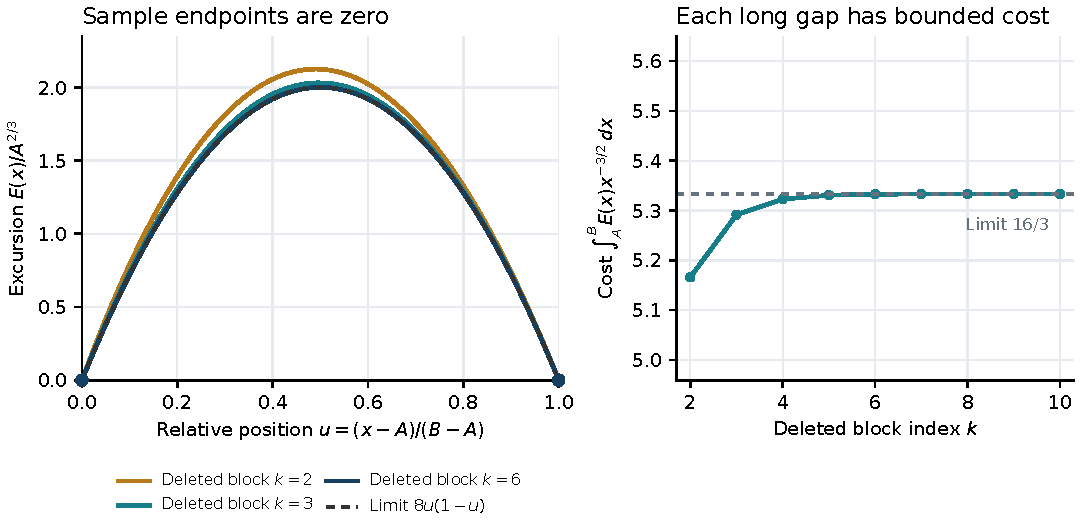
\includegraphics[width=0.93\linewidth]{figures/deleted_block_defect.pdf}
\caption{The extremizing chord defect on the explicit deleted blocks.
The sample errors are zero at the endpoints. After normalization, the
peak approaches \(2\), whereas the weighted cost approaches \(16/3\).
The plotted functions are artificial extremizers, not measurements of
prime-distribution errors.}
\label{fig:defect}
\end{figure}

\subsection{The gap-frequency law}

For a target exponent \(\theta\), a gap of length \(\Delta\asymp X^\alpha\),
with \(\alpha<1\), costs order \(X^{3\alpha-\theta-2}\). If a dyadic
shell \([X,2X]\) contains at most \(O(X^\kappa)\) gaps of this size,
their total cost is bounded at the critical scale whenever
\begin{equation}\label{eq:gap-frequency}
 \boxed{\kappa+3\alpha\leq\theta+2.}
\end{equation}
This is a sufficient budget condition for these gaps. Any remaining
gaps must also have controlled total cost. Summing bounded costs over
dyadic shells gives \(O(\log X)\).

For a regularly spaced mesh with gaps \(X^\alpha\), there are
\(X^{1-\alpha}\) gaps per shell. Substituting
\(\kappa=1-\alpha\) recovers the established scale
\(\alpha\leq(1+\theta)/2\). For boundedly many exceptional gaps per
shell, \(\kappa=0\) gives \(\alpha\leq(\theta+2)/3\).

\begin{center}
\begin{tabular}{lll}
\toprule
Sampling pattern & General threshold & At \(\theta=1/2\)\\
\midrule
Regular gaps throughout a shell & \((1+\theta)/2\) & \(3/4\)\\
Boundedly many exceptional gaps & \((2+\theta)/3\) & \(5/6\)\\
\(O(X^\kappa)\) exceptional gaps & \((2+\theta-\kappa)/3\)
 & \(5/6-\kappa/3\)\\
\bottomrule
\end{tabular}
\end{center}

\begin{figure}[htbp]
\centering
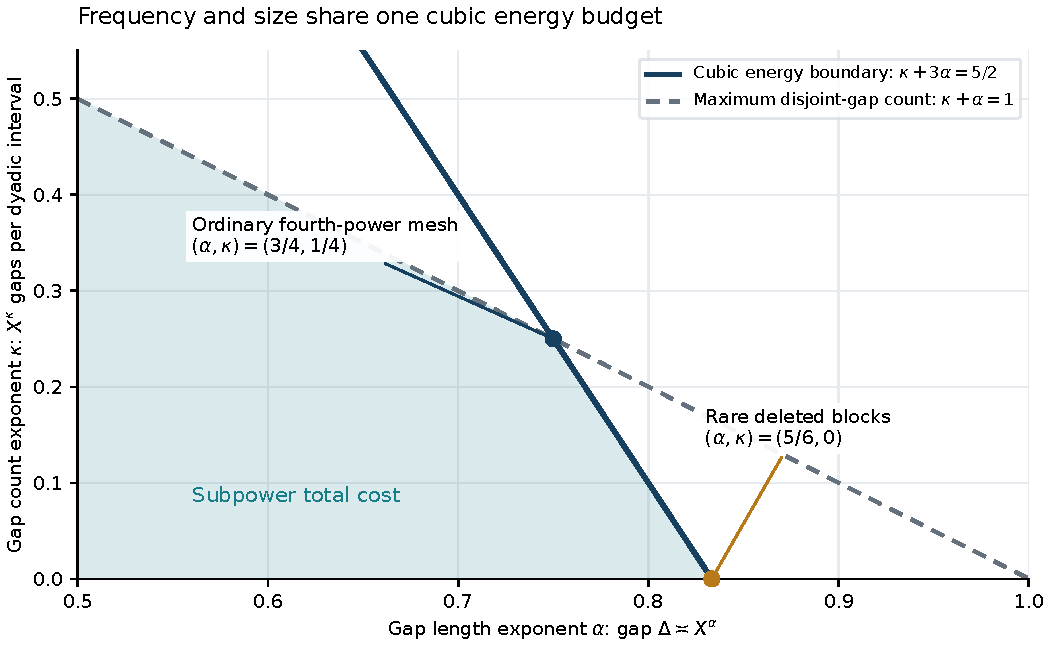
\includegraphics[width=0.84\linewidth]{figures/gap_frequency_budget.pdf}
\caption{The cubic budget at \(\theta=1/2\). Gap length and the number
of such gaps can be traded according to \(\kappa+3\alpha\leq5/2\).
The regular-grid point and isolated-gap point have different frequencies.}
\label{fig:budget}
\end{figure}

The exponent \(5/6\) is sharp for bounded-cost isolated gaps inferred
only from convexity and endpoint values. Indeed, if
\(\alpha>5/6\) is fixed, the exact extremizer incurs a positive power
\(X^{3\alpha-5/2}\) at each such gap. Making the gaps more widely
separated does not make that contribution subpower at the cutoff equal
to its own left endpoint. This observation concerns the interpolation
budget, not every possible zero-free criterion.

\section{From positive-part convergence to absence of poles}
\label{sec:landau}

The following analytic principle is a classical Landau mechanism. A
complete proof is included to make the new sampling implication
self-contained. The upstream proof uses the same real-abscissa idea
\cite{landau}; more general positive-part and oscillation arguments are
well established \cite{brs,odesky}.

\begin{lemma}[Landau's real-abscissa principle]\label{lem:landau}
Let \(f\geq0\) be locally integrable on \([1,\infty)\), with
\(N(s)=\int_1^\infty f(x)x^{-s-1}\dd x\) convergent in some right
half-plane. If its real abscissa of convergence \(\alpha\) is finite,
then \(N\) has no holomorphic continuation to a neighborhood of
the real point \(\alpha\).
\end{lemma}
\begin{proof}
Suppose it had such a continuation on \(B(\alpha,r)\), with \(r>0\).
Take \(s_0=\alpha+r/4\). A Taylor disk around \(s_0\) of radius
\(3r/4\) lies in this continuation disk. For every integer \(m\geq0\),
\[
 (-1)^mN^{(m)}(s_0)
 =\int_1^\infty f(x)(\log x)^m x^{-s_0-1}\dd x\geq0.
\]
Differentiation is justified by convergence at a real parameter strictly
between \(\alpha\) and \(s_0\). Evaluate the Taylor series at
\(s_0-h\), with \(h=r/2\). Its nonnegative integral terms allow
Tonelli's theorem:
\begin{align*}
 N(s_0-h)
 &=\sum_{m=0}^\infty\frac{h^m}{m!}
       \int_1^\infty f(x)(\log x)^m x^{-s_0-1}\dd x\\
 &=\int_1^\infty f(x)x^{-s_0-1}
       \sum_{m=0}^\infty\frac{(h\log x)^m}{m!}\dd x\\
 &=\int_1^\infty f(x)x^{-(s_0-h)-1}\dd x<\infty.
\end{align*}
But \(s_0-h=\alpha-r/4<\alpha\), a contradiction.
\end{proof}

\begin{theorem}[One-sided pole exclusion]\label{thm:poles}
Let \(E\) be real and locally integrable on \([1,\infty)\). Assume:
\begin{enumerate}
\item \(\Mell E(s)=\int_1^\infty E(x)x^{-s-1}\dd x\) converges
absolutely in some right half-plane and continues meromorphically to
\(\Rea s>\theta\);
\item every pole in that domain has order at most one;
\item at every real \(t>\theta\), the residue of the continuation
is nonnegative, interpreting the residue at a regular point as zero;
\item \(\int_1^\infty E(x)_+x^{-\sigma-1}\dd x<\infty\) for all
real \(\sigma>\theta\).
\end{enumerate}
Then \(\Mell E\) is holomorphic throughout \(\Rea s>\theta\).
In particular, the sampling hypotheses of Theorem~\ref{thm:transfer}
or Theorem~\ref{thm:errors} imply this conclusion whenever the first
three analytic assumptions hold.
\end{theorem}

\begin{proof}
Let \(P=\Mell(E_+)\) and \(N=\Mell(E_-)\), where
\(E_-:=(-E)_+\). The function \(P\) is holomorphic on the asserted
half-plane. Far to the right, absolute convergence gives
\(N=P-\Mell E\); this identity supplies a meromorphic continuation
of \(N\) to \(\Rea s>\theta\).

Let \(\alpha\) be the real abscissa of convergence of \(N\).
If \(\alpha\leq\theta\), both \(P,N\) are holomorphic in the desired
half-plane, so the identity theorem finishes the proof. The same holds
if \(\alpha=-\infty\).

Suppose instead that \(\alpha>\theta\). The continuation of \(N\)
has at most a simple pole at \(\alpha\), with residue
\(-\Res_{s=\alpha}\Mell E(s)\leq0\). A strictly negative residue
would force \(N(\sigma)\to-\infty\) as \(\sigma\downarrow\alpha\)
from the right, contradicting its nonnegative integral representation.
A zero residue makes this at-most-simple singularity removable.
That contradicts Lemma~\ref{lem:landau}. Hence \(\alpha\leq\theta\).
\end{proof}

Because \(E\) is real, its meromorphic continuation is invariant under
complex conjugation; real-point residues are real. The condition on
real parts of residues used by the Lean theorem is therefore equivalent
to the real nonnegativity condition above.

\subsection{Why the analytic hypotheses matter}

They cannot be removed just because the positive part is small. For
\(\alpha>\theta\), the function \(E(x)=-x^\alpha\) has \(E_+=0\),
but its Mellin transform is \(-1/(s-\alpha)\), with negative residue.
Likewise \(E(x)=-x^\alpha\log x\) has \(E_+=0\) and transform
\(-1/(s-\alpha)^2\); its residue is zero, but it has a double pole.
These examples explain the sign and simple-pole assumptions. They are
examples for the analytic lemma, without an assertion that their
centered ramp sums have the convexity required elsewhere.

\section{A complete specialization to the zeta function}
\label{sec:zeta}

Define the centered prime ramp sum
\begin{equation}\label{eq:zeta-error}
 E_\zeta(x)=\sum_{n\leq x}\Lambda(n)(x/n-1)
             -x\log x+(1+\gamma)x,\qquad x\geq1,
\end{equation}
where \(\gamma\) is Euler's constant. Its ramp part is convex and
\(a=1\). The centering in \eqref{eq:zeta-error} is essential.

\begin{corollary}[A deleted-sample criterion for RH]\label{cor:zeta}
On the retained fourth-power mesh of Theorem~\ref{thm:deletion}, suppose
\begin{equation}\label{eq:zeta-sampled}
 E_\zeta(x_j)\leq C_\ep x_j^{1/2+\ep}
 \quad\hbox{eventually for every }\ep>0.
\end{equation}
Then \(\zeta(s)\neq0\) for \(\Rea s>1/2\), apart from the pole at
\(s=1\); the functional equation gives RH. More generally, any mesh
satisfying \eqref{eq:headline-energy} and the corresponding sampled
bound at \(1/2\leq\theta<1\) excludes zeros with \(\Rea s>\theta\).
\end{corollary}
\begin{proof}
For \(\Rea s>1\), termwise integration is justified by absolute
convergence and gives
\[
 \int_n^\infty(x/n-1)x^{-s-1}\dd x=\frac{n^{-s}}{s(s-1)}.
\]
Since \(\sum_n\Lambda(n)n^{-s}=-\zeta'(s)/\zeta(s)\),
\begin{equation}\label{eq:zeta-Mellin}
 \Mell E_\zeta(s)
 =-\frac{\zeta'(s)}{\zeta(s)s(s-1)}
       -\frac1{(s-1)^2}+\frac{1+\gamma}{s-1}.
\end{equation}
For example, \(\Lambda(n)\leq\log n\) implies the elementary bound
\(E_\zeta(x)=O(x\log^2(2x))\), which also supplies initial absolute
Mellin convergence. The Laurent expansion
\(-\zeta'/\zeta=1/(s-1)-\gamma+O(s-1)\) shows that the singularity
at \(1\) in \eqref{eq:zeta-Mellin} is removable.

Every other possible singularity in \(\Rea s>0\) is a simple pole at
a zeta zero \(\rho\), with residue
\begin{equation}\label{eq:zeta-residue}
 \frac{m_\rho}{\rho(1-\rho)},
\end{equation}
where \(m_\rho\geq1\) is its multiplicity. Multiple zeros still produce
only simple logarithmic-derivative poles.

The zeta function has no positive real zeros. For real \(s>1\), this
follows from its positive Dirichlet series. For \(0<s<1\), the
alternating series
\(\eta(s)=\sum_{n\geq1}(-1)^{n-1}n^{-s}\) is positive: group
successive pairs, or use the alternating-series estimate
\(\eta(s)\geq1-2^{-s}>0\). The identity
\(\eta(s)=(1-2^{1-s})\zeta(s)\) then shows \(\zeta(s)<0\).
Thus the real residues of \eqref{eq:zeta-Mellin} are zero.

The sampling theorem gives convergence of the positive part on
\(\Rea s>\theta\). Theorem~\ref{thm:poles} makes
\eqref{eq:zeta-Mellin} holomorphic there. A zeta zero would have the
nonzero residue \eqref{eq:zeta-residue}, a contradiction. When
\(\theta=1/2\), the usual functional equation reflects a zero to the
left of the critical line to one on its right, giving the last step.
\end{proof}

The Mellin identity and the corresponding uniformly sampled criterion
are established ingredients \cite{setiawan}. The new assertion is that
the explicit growing blocks in \eqref{eq:deleted-indices} can be omitted
from the sampling hypothesis, with the stated sharp integrated cost.
The proof is not a new proof of the arithmetic estimate
\eqref{eq:zeta-sampled}; it is a precise weakening of what a sampling
based derivation needs to establish.

\section{Transfer to the repository's Dirichlet GRH criterion}
\label{sec:dirichlet}

\subsection{Centering and pole multiplicities}

Fix \(q>0\) divisible by \(8\), and an invertible residue class
\(d_0\pmod q\) with \(d_0\equiv7\pmod8\). Let \(d\) run through
primes in this class. For the weights in \eqref{eq:weights}, set
\(W_{d,q}(s)=\sum_nw_{d,q}(n)n^{-s}\), initially for \(\Rea s>1\).
Its Laurent expansion at \(1\) has the form
\begin{equation}\label{eq:W-laurent}
 W_{d,q}(s)=\frac{a}{s-1}+b_{d,q}+O(s-1),\qquad
 a=\frac1{\varphi(q)}.
\end{equation}
Define \(c_{d,q}=b_{d,q}-a\), which is real. This agrees with the
repository's \(\Rea\,\texttt{logDerivMean}\ d\ q\ 1\), because its
Dirichlet-series identity is
\(W_{d,q}(s)=as/(s-1)+\texttt{logDerivMean}\ d\ q\ s\)
\cite{primeerror}.

With \(E_{d,q}=xR_{d,q}\), direct integration gives
\begin{equation}\label{eq:dirichlet-Mellin}
 \Mell E_{d,q}(s)=\frac{W_{d,q}(s)}{s(s-1)}
              -\frac{a}{(s-1)^2}-\frac{c_{d,q}}{s-1}.
\end{equation}
Equation~\eqref{eq:W-laurent} proves removability at \(1\). The source
establishes meromorphic continuation and at-most-simple poles in
\(\Rea s>0\). Away from \(0,1\), their residues are
\begin{equation}\label{eq:dirichlet-residue}
 \frac{\displaystyle\sum_{\chi\bmod q}m_\chi(\rho)
            -\displaystyle\sum_{\chi\bmod q}m_{\chi\chi_d}(\rho)}
       {\varphi(q)\rho(1-\rho)},
\end{equation}
where \(\chi_d(n)=(n/d)\), and \(m_\chi\) is the zero multiplicity
of the entire \(L\)-function obtained by removing the principal pole.
In the open strip these are the ordinary \(L\)-function zero
multiplicities \cite{primeerror}.

\subsection{The sampled transfer theorem}

\begin{theorem}[Cubic-budget transfer for a fixed modulus]\label{thm:dirichlet}
Let \(1/2\leq\theta<1\). Suppose that for every admissible prime
\(d\equiv d_0\pmod q\), there is a mesh \(\mesh_d\) on which:
\begin{enumerate}
\item \(H_\theta(X)=O_\ep(X^\ep)\) for all \(\ep>0\);
\item \(E_{d,q}(x_j)\leq C_{d,\ep}x_j^{\theta+\ep}\) eventually
for every \(\ep>0\).
\end{enumerate}
Then no Dirichlet \(L(s,\chi)\), \(\chi\bmod q\), has a zero in
\(\Rea s>\theta\). The principal pole at \(1\) is understood as a pole.
The constants and meshes may depend on \(d\).
\end{theorem}
\begin{proof}
Theorem~\ref{thm:transfer} gives positive-part Mellin convergence for
each admissible \(d\) throughout \(\Rea s>\theta\).
Suppose \(L(\rho,\psi)=0\) with \(\Rea\rho>\theta\).
The Euler product and the established boundary nonvanishing reduce the
issue to \(\theta<\Rea\rho<1\). Choose
\(\max(\theta,1/2)<\beta<\Rea\rho\).

The repository's quadratic-twist avoidance theorem supplies an
admissible \(d\) such that every twisted \(L(s,\chi\chi_d)\) is
nonzero for
\(\Rea s\geq\beta\), \(|\Ima s|\leq|\Ima\rho|\)
\cite{twist,criterion}. This region includes all real points
\(t\geq\beta\). Thus, for \(\beta<t<1\),
\eqref{eq:dirichlet-residue} is nonnegative. At \(t=1\) the
singularity is removable, and at \(t>1\) there are no zeros or poles.

Theorem~\ref{thm:poles} now applies to the selected \(d\), on
\(\Rea s>\beta\). At \(\rho\), all twisted multiplicities vanish,
whereas \(\sum_\chi m_\chi(\rho)\geq m_\psi(\rho)\geq1\).
The residue \eqref{eq:dirichlet-residue} is nonzero, contradicting
holomorphy. This excludes the candidate zero.
\end{proof}

In particular, the same deleted fourth-power mesh works for every
\(d\) at \(\theta=1/2\). If the corresponding sampled estimates are
available for every modulus, functional equations give Dirichlet GRH.
The original arithmetic construction uses a larger modulus divisible by
\(18480\); induction of characters supplies arbitrary original moduli
\cite{onesided}. The sampling refinement can be inserted at that
existing interface.

\subsection{An optional sparse set of auxiliary primes}

There is a second, independent sparsity available from the code. For
fixed \(\beta>1/2\) and height \(H\), its twist-density estimate bounds
the number of unsuitable primes \(d\leq Y\) by
\begin{equation}\label{eq:bad-twists}
 O_{q,\beta,H}\left(Y^{\gamma_\beta}\right),\qquad
 \gamma_\beta=1-\frac{\beta-1/2}{18}.
\end{equation}
This is the exponent obtained from \(\beta=1/2+9\delta\) and the
bound \(O(Y^{1-\delta/2})\) in the source \cite{twist}.

\begin{corollary}[Sparse auxiliary-prime transfer]\label{cor:sparse-d}
Fix \(1/2<\beta<1\). It is enough to establish positive-part Mellin
convergence on \(\Rea s>\beta\), by either cubic-budget theorem, for
an admissible set \(S\) of auxiliary primes satisfying
\begin{equation}\label{eq:sparse-S}
 \limsup_{Y\to\infty}
 \frac{\#\{d\in S:d\leq Y\}}{Y^{\gamma_\beta}}=\infty.
\end{equation}
Then all characters modulo \(q\) are zero-free in \(\Rea s>\beta\).
\end{corollary}
\begin{proof}
For every fixed height \(H\), the set in \eqref{eq:sparse-S} cannot
be contained in the unsuitable set bounded by \eqref{eq:bad-twists}.
Choose a suitable member of \(S\) and repeat the residue argument in
Theorem~\ref{thm:dirichlet}.
\end{proof}

If \(S\) has upper counting exponent
\(\tau=\limsup_{Y\to\infty}\log\max(1,\#S\cap[1,Y])/\log Y\), a
sufficient condition is
\(\beta>1/2+18(1-\tau)\), with \(\beta\in(1/2,1)\).
Equality is not justified by this density estimate. Upper counting
exponent \(1\) suffices for every \(\beta>1/2\). This corollary is a
direct extraction from the existing zero-density bound and is not the
principal novelty claim of this note.

\section{Prior work, novelty, and verification}
\label{sec:status}

\subsection{What the literature already contains}

The requested Wikipedia article lists familiar consequences and
equivalent criteria for RH \cite{wiki}. Our research did not select one
of those consequences and relabel it as new. Instead, it followed the
specific one-sided analytic interface in the repository.

The closest result located is Setiawan's \emph{The Primacohedron Trace
Formulation of the Riemann Hypothesis}, version 2, posted
25 November 2026 \cite{setiawan}. It proves a pointwise sampling theorem
with maximum gaps \(O(X^{(1+\theta)/2})\), a localized fourth-power
criterion, and a signed dyadic-average criterion. Our criterion uses
global eventual sample control but permits larger isolated gaps through
a total integrated budget. Neither formulation dominates the other in
all respects: the cited theorem permits control only on arbitrarily
late intervals, whereas our stated sampling hypothesis is eventual on
the retained infinite mesh.

Landau's real convergence-abscissa principle is classical
\cite{landau}. Positive-part Mellin methods and localized oscillation
arguments predate the current RH work \cite{brs}. The original
Alp\"oge development also has a localized endpoint allowing integral
majorants, discussed in \cite{odesky}. We therefore make no novelty
claim for replacing a pointwise majorant by an integrable one in
isolation. Finally, the \(h^3/12\) local error is a classical
quadrature fact \cite{dlmf}.

\subsection{The precise claim of originality}

The contribution established here is the following combination:
\begin{enumerate}
\item a total cubic mesh-energy hypothesis that transfers one-sided
sample control to positive-part Mellin convergence;
\item an exact global optimum for the integrated reconstruction error,
attained simultaneously on all gaps by a nonnegative arithmetic weight
sequence;
\item an explicit fourth-power mesh with infinitely many growing
deleted blocks and gaps \(\sim4X^{5/6}\), whose critical total budget
is only \(O(\log X)\);
\item the resulting insertion into the one-sided zeta and Dirichlet
\(L\)-function pole-exclusion arguments.
\end{enumerate}
Targeted searches for cubic total-gap conditions, positive-part Mellin
sampling, missing fourth-power blocks, and the isolated \(5/6\) scale
found no identical statement in the checked primary sources. This is a
\emph{proved refinement that appears new relative to that search}, not a
certification of historical priority. The proof does not assert the
resolution of an additional named open conjecture.

\subsection{Computational and formal verification status}

The proof of the new theorem is the analytic argument in this note.
The accompanying program checks its formulas and finite examples:
\begin{itemize}
\item symbolic differentiation of the chord defect and the local
\(1/12\) expansion;
\item 100-digit comparisons of \eqref{eq:J-half} with independent
numerical quadrature for four intervals;
\item a nonnegative integer-supported extremizer and its sample and
interior identities;
\item exact integer expansions and inequalities for the omitted
fourth-power blocks;
\item finite mesh-energy calculations and the two figures.
\end{itemize}
The largest relative discrepancy in the four quadrature comparisons
was approximately \(6.47\times10^{-83}\). These calculations are
supplementary verification, not a numerical proof of an infinite
statement. At \(k=10\), for example, the table gives
\[
 \frac{\Delta_k}{A_k^{5/6}}\approx4.000005722,
 \quad J_{1/2}(A_k,B_k)\approx5.333330790,
 \quad\frac{\max d_{A_k,B_k}}{A_k^{2/3}}\approx2.000001907.
\]
The limiting values \(4\), \(16/3\), and \(2\) have proofs above.

The source manifest records the inspected repository revision, paths,
and blob identifiers. No Lean or Lake executable was available in the
working environment, so neither the upstream project nor a new Lean
formalization was compiled. The file \path{formalization/outline.txt}
specifies a route through convexity, interval integration, summability,
holomorphic parameter integrals, and the strengthened Landau interface.
It is explicitly a design outline, not a completed formal proof.

\subsection{How to reproduce the supporting artifacts}

The archive contains the complete LaTeX source and compiled PDF. From
the extracted directory, install the Python dependencies listed in
\path{code/requirements.txt} if needed and run
\begin{quote}\ttfamily
python3 code/verify.py
\end{quote}
This regenerates \path{code/verification_results.json},
\path{code/gap_table.csv}, and the figure files. A standard TeX Live
installation can rebuild the report using \path{build.sh}.
The source needs no external figures beyond those included in the
archive and no network access to compile.

\appendix
\section{A compact statement for reuse}

For applications, the entire refinement can be packaged as follows.

\begin{theorem}[Reusable analytic interface]\label{thm:reuse}
Let \(0\leq\theta<1\), and let \(E=C-ax\log x-cx\), with \(a>0\),
\(C\) convex, and \(E\) real and locally integrable. Suppose its Mellin
transform initially converges absolutely, continues meromorphically to
\(\Rea s>\theta\), has only simple poles there, and has nonnegative
residue at each real point \(t>\theta\). If an unbounded increasing
mesh satisfies
\[
 E(x_j)\leq C_\ep x_j^{\theta+\ep},\qquad
 \sum_{x_j\leq X}\frac{(x_{j+1}-x_j)^3}{x_j^{\theta+2}}
       \leq K_\ep X^\ep
\]
eventually for every \(\ep>0\), then the Mellin transform is
holomorphic on \(\Rea s>\theta\).
\end{theorem}
\begin{proof}
Combine Theorems~\ref{thm:transfer} and~\ref{thm:poles}.
\end{proof}

In a number-theoretic application, the essential extra work is to show
that a zero one wants to exclude would produce a nonzero residue of
this transform, and to establish the real-residue condition. For zeta,
Section~\ref{sec:zeta} supplies this directly. For the repository's
Dirichlet sums, Section~\ref{sec:dirichlet} supplies it after choosing a
quadratic twist.

\section{Source locations}

The following table identifies the exact modules used. All paths are
relative to \path{grh/src/} in the pinned repository revision.
The archive's source manifest supplies the full URLs and blob hashes.

\begin{center}\small
\begin{tabular}{p{0.47\linewidth}p{0.45\linewidth}}
\toprule
Module & Role\\
\midrule
\path{Statements.lean}; \path{Main.lean}
 & Public RH and Dirichlet GRH statements\\[3pt]
\path{New/Reduction/MainInequality.lean}
 & Arithmetic comparison and main-term cancellation\\[3pt]
\path{New/Reduction/OneSidedBound.lean}
 & Eventual upper bound for the prime remainder\\[3pt]
\path{New/Reduction/Zeros/PrimeError.lean}
 & Centering, Mellin transform, polar residues\\[3pt]
\path{Lib/Analytic/Landau.lean}
 & Positive-transform convergence-abscissa argument\\[3pt]
\path{Lib/Analytic/QuadraticTwist.lean}
 & Zero-density bound and auxiliary twist selection\\[3pt]
\path{New/Reduction/Zeros/Criterion.lean}
 & Final zero-free criterion\\
\bottomrule
\end{tabular}
\end{center}

\begin{thebibliography}{99}\small\raggedright
\bibitem{repo}
L. Sernau and collaborators, \emph{GRH for Dirichlet L-functions, in
Lean 4}, repository README, pinned revision
\texttt{72fead102f663d5c7a407964a13dc0cf9d977207}, 25 November 2026.
\url{https://github.com/lsernau/grh-lean}.

\bibitem{guide}
Same repository, \path{grh/GUIDE.md}, at the pinned revision.
\url{https://github.com/lsernau/grh-lean/blob/72fead102f663d5c7a407964a13dc0cf9d977207/grh/GUIDE.md}.

\bibitem{statements}
Same repository, \path{grh/src/Statements.lean}, at the pinned revision.
\url{https://github.com/lsernau/grh-lean/blob/72fead102f663d5c7a407964a13dc0cf9d977207/grh/src/Statements.lean}.

\bibitem{main}
Same repository, \path{grh/src/Main.lean}, at the pinned revision.
\url{https://github.com/lsernau/grh-lean/blob/72fead102f663d5c7a407964a13dc0cf9d977207/grh/src/Main.lean}.

\bibitem{mainineq}
Same repository, \path{grh/src/New/Reduction/MainInequality.lean},
especially \texttt{star\_inequality}.
\url{https://github.com/lsernau/grh-lean/blob/72fead102f663d5c7a407964a13dc0cf9d977207/grh/src/New/Reduction/MainInequality.lean}.

\bibitem{onesided}
Same repository, \path{grh/src/New/Reduction/OneSidedBound.lean},
especially \texttt{eventually\_primeRemainder\_le\_rpow}.
\url{https://github.com/lsernau/grh-lean/blob/72fead102f663d5c7a407964a13dc0cf9d977207/grh/src/New/Reduction/OneSidedBound.lean}.

\bibitem{primeerror}
Same repository, \path{grh/src/New/Reduction/Zeros/PrimeError.lean},
especially \texttt{primeRemainder}, \texttt{integral\_primeRemainder},
and \texttt{isPolar\_primeRemainder}.
\url{https://github.com/lsernau/grh-lean/blob/72fead102f663d5c7a407964a13dc0cf9d977207/grh/src/New/Reduction/Zeros/PrimeError.lean}.

\bibitem{landau}
Same repository, \path{grh/src/Lib/Analytic/Landau.lean},
especially \texttt{IsPolar.landau}; the file cites Montgomery--Vaughan,
\emph{Multiplicative Number Theory I} (2007), Lemma 15.1, and Widder,
\emph{The Laplace Transform} (1941), II Theorem 5b.
\url{https://github.com/lsernau/grh-lean/blob/72fead102f663d5c7a407964a13dc0cf9d977207/grh/src/Lib/Analytic/Landau.lean}.

\bibitem{twist}
Same repository, \path{grh/src/Lib/Analytic/QuadraticTwist.lean},
especially \texttt{zero\_density\_quadTwist} and
\texttt{exists\_entireL\_quadTwist\_ne\_zero}.
\url{https://github.com/lsernau/grh-lean/blob/72fead102f663d5c7a407964a13dc0cf9d977207/grh/src/Lib/Analytic/QuadraticTwist.lean}.

\bibitem{criterion}
Same repository, \path{grh/src/New/Reduction/Zeros/Criterion.lean},
especially \texttt{New.LFunction\_ne\_zero\_of\_primeRemainder\_le}.
\url{https://github.com/lsernau/grh-lean/blob/72fead102f663d5c7a407964a13dc0cf9d977207/grh/src/New/Reduction/Zeros/Criterion.lean}.

\bibitem{wiki}
Wikipedia contributors, \emph{Riemann hypothesis}, accessed
26 November 2026. Used for orientation and the requested source review.
\url{https://en.wikipedia.org/wiki/Riemann_hypothesis}.

\bibitem{leancommunity}
Lean FRO and Mathlib Initiative, \emph{Lean verification of the Riemann
Hypothesis}, 21 November 2026.
\url{https://leanprover-community.github.io/blog/posts/riemann-hypothesis/}.

\bibitem{setiawan}
S. Setiawan, \emph{The Primacohedron Trace Formulation of the Riemann
Hypothesis: A Guide to Reconstructing the Alp\"oge--Claude Proof in Lean},
version 2, posted 25 November 2026, preprint (not peer reviewed).
\url{https://doi.org/10.20944/preprints202611.0738.v2}.
Publisher record: \url{https://www.preprints.org/manuscript/202611.0738}.
Full-text version consulted:
\url{https://www.academia.edu/181628231/The_Primacohedron_Trace_Formulation_of_the_Riemann_Hypothesis_A_Guide_to_Reconstructing_the_Alp%C3%B6ge_Claude_Proof_in_Lean}.

\bibitem{dlmf}
NIST Digital Library of Mathematical Functions, Section 3.5(i),
equation 3.5.1, elementary trapezoidal rule.
\url{https://dlmf.nist.gov/3.5.E1}.

\bibitem{brs}
G. Bhowmik, O. Ramar\'e, and J.-C. Schlage-Puchta,
\emph{Tauberian Oscillation Theorems and the Distribution of Goldbach
numbers}, Journal de th\'eorie des nombres de Bordeaux
\textbf{28} (2016), no. 2, 291--299.
\url{https://doi.org/10.5802/jtnb.940}.
\url{https://www.numdam.org/item/JTNB_2016__28_2_291_0/}.

\bibitem{odesky}
A. O'Desky, \emph{Landau theorem on intervals}, exposition of the
Alp\"oge Lean development, version 9, 24 November 2026.
\url{https://andrewodesky.com/rh/lean/Deduction.zeroFree_of_rpow_window/}.
\end{thebibliography}
\end{document}


